\documentclass{article}

% NeurIPS 2026 double-blind workshop submission format. Replace the workshop
% title below with the exact title used by the target workshop.
\usepackage[dblblindworkshop]{neurips_2026}
\workshoptitle{NeurIPS 2026 Workshop}

\usepackage[utf8]{inputenc} % allow UTF-8 input
\usepackage[T1]{fontenc}    % use 8-bit T1 fonts
\usepackage{hyperref}
\usepackage{url}
\usepackage{booktabs}
\usepackage{amsfonts}
\usepackage{amsmath}
\usepackage{amssymb}
\usepackage{graphicx}
\usepackage{nicefrac}
\usepackage{microtype}
\usepackage{tabularx}
\usepackage{array}
\usepackage{tikz}
\usepackage{xcolor}
\usepackage{placeins}
\usetikzlibrary{arrows.meta,fit,positioning}

\newcommand{\benchmark}{\textsc{DUAL-AudioBench}}
\newcommand{\numscenarios}{84}
\newcommand{\numpairs}{42}
\newcommand{\numdomains}{14}
\newcommand{\numconditions}{9}
\newcolumntype{Q}[1]{>{\raggedright\arraybackslash}p{#1}}
\newcolumntype{Z}{>{\raggedright\arraybackslash}X}
\newcommand{\dualcolhead}[1]{\textbf{#1}}

% Eight-page main-text budget with the official NeurIPS style:
% abstract/introduction 1.25 pages; related work 1.0; methods 2.5;
% results and analysis 2.5; limitations/conclusion 0.75. Move expanded
% scenario examples, prompts, audit forms, and metric definitions to appendices.

\title{\benchmark: Closed-Loop Evaluation of Belief-State Synchronization in Audio-Conditioned Conversational Agents}

% Keep the submission anonymous for double-blind workshop review.
\author{Anonymous Authors}

\begin{document}

\maketitle

\begin{abstract}
Reliable voice agents must update their view of the world when their actions, elapsed time, external events, or users change it. Current evaluations measure spoken task completion, interruption handling, and stateful tool use, yet rarely reveal whether an agent's internal belief follows a delayed hidden transition. We introduce \benchmark, a turn-based audio-replay benchmark for long horizon state synchronization evaluation in voice agents. Each evaluation run places an agent in a deterministic environment, executes its first action, advances simulated time, and then  resumes with a spoken observation that leaves the new state partly implicit. The benchmark contains \numscenarios{} scenarios organized into \numpairs{} matched causal pairs across \numdomains{} domains and three clue distances. Within each pair, one early fact changes the terminal state and correct final action with fixed post-gap words and action menus. Models report probabilities over possible states before and after the gap, allowing belief updating to be measured separately from action choice. Across 4,368 completed trajectories with three audio-capable models, first-action accuracy under audio replay ranged from 65.5\% to 80.4\%, but final-action accuracy after the hidden transition ranged from 22.0\% to 47.0\%. Suppressing the transition improved immediate state estimates by 21.4--32.1 points, whereas moving the clue close to the decision did not help. Explicitly stating the changed state improved final-action accuracy by 32.7--41.1 points. These controls pinpoint the main difficulty as inferring an unobserved transition instead of retaining the clue alone.
\end{abstract}

\section{Introduction}

Voice agents increasingly make decisions that change external systems. The result of an action may remain unobserved while a maintenance job runs, a transaction settles, or a user independently modifies the same account. When dialogue resumes, the agent must infer the current state before choosing its next action. Final task success alone cannot show whether the agent tracked the transition: the same endpoint can arise from a calibrated decision, a lucky guess, or a stale belief paired with an inconsistent action.

Audio-language benchmarks cover acoustic understanding, paralinguistics, long recordings, and multi-turn memory \citep{yang2024airbench,wang2024audiobench,li2026wavbench,gosa2025audiomultichallenge}. VoiceAgentBench adds multilingual tool invocation and adversarial spoken queries \citep{jain2025voiceagentbench}. Full-duplex evaluations measure timing, overlap, correction, and interruption \citep{lin2025fullduplex,lin2025fullduplexv2,ge2025flexi}. EchoChain is the closest state-update benchmark: it tests whether an agent revises an ongoing response after a user interrupts mid-speech \citep{modi2026echochain}. Its target is online revision during concurrent speech. Our target is cross-gap inference after an action-dependent world transition, with the agent's probability distribution and chosen action scored against the same executable state.

Executable agent benchmarks verify tool calls against state changes rather than relying only on response judgments \citep{lu2024toolsandbox,yao2024taubench,barres2025tau2}. Recent voice benchmarks extend this idea to grounded, end-to-end calls: $\tau$-Voice combines full-duplex speech with real-world tools and policies, EVA-Bench evaluates task accuracy and interaction quality across enterprise scenarios, and VAmoS verifies voice-agent behavior against an isolated database \citep{ray2026tauvoice,bogavelli2026evabench,meyer2026vamos}. These evaluations provide greater interaction and deployment realism. \benchmark concentrates measurement on one mechanism---synchronizing belief after delayed, partially observed change---using matched counterfactuals and explicit probability reports.

\benchmark contains \numscenarios{} scenarios arranged as \numpairs{} matched pairs: \numdomains{} domains $\times$ three clue-distance buckets $\times$ two causal branches. Each dialogue states a rule and later supplies one fact needed to apply it. In the aligned branch the fact permits completion; in the misaligned branch it creates a recoverable failure. The pair shares fillers, voices, action menus, and post-gap words. Only the early fact changes, causing a different hidden outcome and a different correct final action. Removing that fact makes the paired public histories identical and limits a clue-independent policy to 50\% expected post-gap accuracy.

After the pre-gap action, a deterministic simulator advances task-specific time, applies any user or external event, and generates the resumed observation from the realized state. Probability reports are collected with the first action, immediately after resumption, and with the final action. This reveals whether new evidence moves probability toward the realized state and separates state-estimation failures from action-selection failures.

Our contributions are:
\begin{itemize}
  \item \textbf{A delayed-transition diagnostic.} Symbolic actions alter a deterministic hidden world; elapsed time and external events produce the evidence and correct action for the realized run.
  \item \textbf{Matched causal scenarios.} \numpairs{} pairs change one early fact while holding the resumed utterance and menu fixed, making clue dependence identifiable rather than inferred from correlation.
  \item \textbf{Belief and decision measurement.} Three probabilistic checkpoints expose calibration, revision, stale-state mass, and consistency between beliefs, uncertainty flags, and actions.
  \item \textbf{Controlled audio evaluation.} Nine conditions vary modality, clue distance and removal, external and user-driven change, and spoken delivery with stable menus and inspectable logs.
  \item \textbf{Auditable evaluation.} Fixed transition rules, plain-language action descriptions, shuffled labels, appropriate chance baselines, and inspectable records make failures reproducible and attributable.
\end{itemize}

\paragraph{Scope.}
\benchmark fixes turn boundaries and replays the visible audio history at each model call. Streaming latency, overlap, barge-in, backchannels, and generated voice quality fall outside its evaluation target; EchoChain and the Full-Duplex-Bench family measure those interaction dynamics directly. Here, ``long-horizon'' refers to causal distance across intervening turns and a simulated time gap, rather than a continuously recorded hour-scale waveform. This scope keeps failures attributable to state inference and belief revision.

\section{Related Work}

\paragraph{Audio and multi-turn understanding.}
AIR-Bench, AudioBench, VoiceBench, and WavBench evaluate broad audio comprehension, speech variation, reasoning, and paralinguistics \citep{yang2024airbench,wang2024audiobench,chen2024voicebench,li2026wavbench}. BLAB and AudioMarathon study physically long recordings \citep{ahia2025blab,he2025audiomarathon}. SpokenWOZ supplies dialogue-state annotations, while Audio MultiChallenge and MTalk-Bench target multi-turn memory, consistency, natural conversation, and acoustic cues \citep{si2023spokenwoz,gosa2025audiomultichallenge,du2025mtalk}. VoiceAgentBench adds multilingual, multi-tool, multi-turn, safety, and adversarial spoken tasks \citep{jain2025voiceagentbench}. AudioAgentBench (Audio Arena) uses fixed multi-turn audio to grade tool use, grounding, state tracking, ambiguity handling, and turn taking across customer-facing domains \citep{arcadalabs2026audioarena}. These benchmarks establish breadth across audio and dialogue phenomena. \benchmark adds an action-conditioned simulator and scores the model's probability distribution over the resulting state.

Belief-state representations are well established in task-oriented dialogue, and recent agent work uses explicit uncertainty to separate state estimation from policy learning \citep{si2023spokenwoz,singh2026agentbrace}. \benchmark uses the same conceptual separation as an evaluation instrument: the reported distribution is scored at fixed points before and after an executable transition, without training a separate belief model.

\paragraph{Paralinguistic controls.}
Recent evaluations show that audio access does not guarantee use of vocal affect, and matched-transcript speech delivery can change model behavior \citep{ayllon2026voiceeq,qian2026pjbreak}. These results make prosody an important control, but they also set a high validation standard: the acoustic manipulation must first be recognizable independently of model behavior. We therefore treat our spoken-delivery conditions as exploratory until the listening audit is complete.

\paragraph{Real-time state revision.}
Full-Duplex-Bench and its later versions evaluate turn-taking, pacing, corrections, entity tracking, disfluency, and tool use in streaming interaction \citep{lin2025fullduplex,lin2025fullduplexv2,lin2026fullduplexv3}. MTR-DuplexBench broadens the setting to multi-round instruction following and safety, and FLEXI studies latency, conversational effectiveness, and emergency interruption \citep{zhang2025mtrduplex,ge2025flexi}. EchoChain most directly overlaps our state-update motivation. It injects a user interruption during assistant speech and diagnoses whether the continuation incorporates the new objective, using a paired half-duplex control \citep{modi2026echochain}. EchoChain therefore measures online revision of an answer already in progress. \benchmark measures revision of an explicit world-state distribution after the agent acts and the environment evolves during a gap. The two benchmarks expose different synchronization failures and can be used together.

\paragraph{Grounded voice agents and executable state.}
ToolSandbox, $\tau$-bench, and $\tau^2$-bench verify conversational tool use against executable state; the last allows the user and agent to modify a shared environment \citep{lu2024toolsandbox,yao2024taubench,barres2025tau2}. $\tau$-Voice adds full-duplex interaction, realistic acoustics, policies, and grounded task completion \citep{ray2026tauvoice}. EVA-Bench evaluates complete voice systems through simulated enterprise calls, task and experience metrics, and acoustic perturbations \citep{bogavelli2026evabench}. VAmoS uses isolated database instances and trace-level assertions to test containment and policy compliance \citep{meyer2026vamos}. These systems more closely approximate deployed calls. \benchmark uses a smaller controlled world so that one changed clue can be tied to a different hidden outcome, gold action, and belief target. By utilizing mechanism-level attribution, it distinguishes failure to infer state from failure to act on a correct inference.

\begin{table*}[t]
  \centering
  \footnotesize
  \setlength{\tabcolsep}{4.5pt}
  \renewcommand{\arraystretch}{1.12}
  \caption{Closest benchmark families and their primary diagnostic target. ``State evidence'' identifies what supports a success or failure judgment.}
  \label{tab:positioning}
  \begin{tabularx}{\textwidth}{@{}Q{0.18\textwidth}Q{0.22\textwidth}Q{0.23\textwidth}Z@{}}
    \toprule
    \dualcolhead{Benchmark} & \dualcolhead{Primary target} & \dualcolhead{State evidence} & \dualcolhead{Controlled contrast} \\
    \midrule
    Audio MultiChallenge / MTalk \citep{gosa2025audiomultichallenge,du2025mtalk}
      & Spoken memory and acoustic cues & Human rubrics / response judgments & Conversation and cue categories \\
    VoiceAgentBench \citep{jain2025voiceagentbench}
      & Multilingual spoken tool use and safety & Tool-call correctness & Language, workflow, adversarial query \\
    AudioAgentBench \citep{arcadalabs2026audioarena}
      & Long multi-turn voice-agent behavior & Per-turn category judgments & Domain, TTS vs. human audio \\
    Full-Duplex-Bench / FLEXI \citep{lin2025fullduplexv2,ge2025flexi}
      & Streaming timing, correction, interruption & Interaction trace and task scores & Pacing and interruption setting \\
    EchoChain \citep{modi2026echochain}
      & State revision during mid-speech interruption & Instance rubric and human review & Interrupted vs. paired half-duplex \\
    $\tau$-Voice \citep{ray2026tauvoice}
      & Grounded full-duplex task completion & Executable environment and policy & Text vs. voice; acoustic conditions \\
    EVA-Bench / VAmoS \citep{bogavelli2026evabench,meyer2026vamos}
      & End-to-end task quality and containment & Composite metrics / database assertions & Acoustic perturbation / adversarial caller \\
    \textbf{\benchmark}
      & Delayed belief-state synchronization & Simulator state, belief distribution, and action & Matched clue branch, ablation, and gap controls \\
    \bottomrule
  \end{tabularx}
\end{table*}

The defining combination in \benchmark is a matched clue intervention that changes an executable terminal state, an implicit post-gap observation, and probability reports scored against the state before and after the transition. This design supports causal claims about clue use and separates belief updating from action selection. The other benchmarks in Table~\ref{tab:positioning} provide complementary evidence about audio robustness, natural interaction, and end-to-end task reliability.

\section{Methods}

Figure~\ref{fig:pipeline} gives the complete evaluation loop. The blue stages are visible to the model and follow half-duplex turn taking: one participant speaks at a time. The gray stage is the hidden simulator. It executes the model's action, advances time, and uses the resulting state to produce the next spoken observation and answer key.

\begin{figure*}[t]
  \centering
  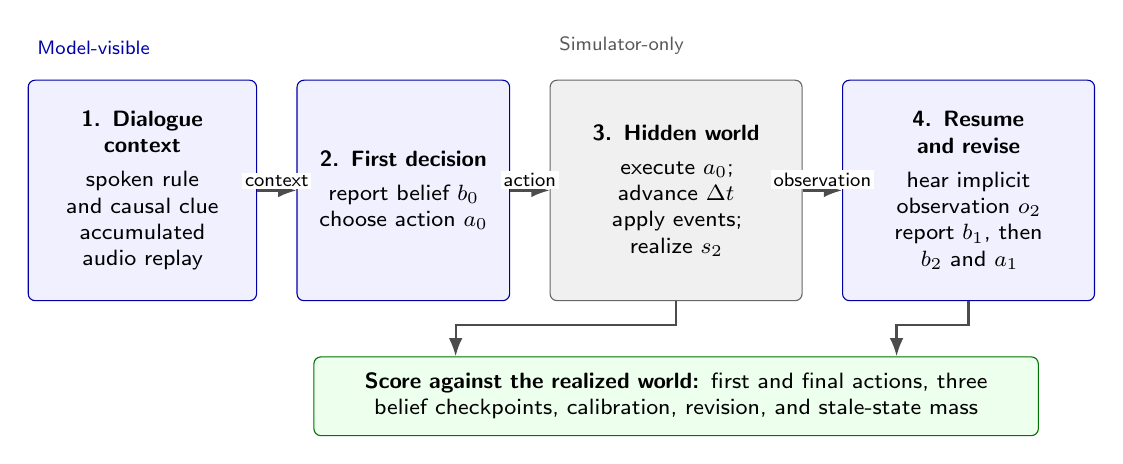
\begin{tikzpicture}[
    font=\sffamily\footnotesize,
    >=Latex,
    stage/.style={
      draw,
      rounded corners=2.5pt,
      align=center,
      minimum height=28mm,
      inner xsep=2.5mm,
      inner ysep=2mm
    },
    visible/.style={stage, draw=blue!65!black, fill=blue!6},
    hidden/.style={stage, draw=black!60, fill=black!6},
    score/.style={
      draw=green!45!black,
      fill=green!7,
      rounded corners=2.5pt,
      align=center,
      minimum height=10mm,
      inner xsep=3mm
    },
    flow/.style={->, thick, draw=black!70},
    flowlabel/.style={font=\sffamily\scriptsize, fill=white, inner sep=1pt}
  ]
    \node[visible, text width=24mm] (context)
      {\textbf{1. Dialogue context}\\[1mm]spoken rule and causal clue\\accumulated audio replay};
    \node[visible, text width=22mm, right=5mm of context] (decision)
      {\textbf{2. First decision}\\[1mm]report belief $b_0$\\choose action $a_0$};
    \node[hidden, text width=27mm, right=5mm of decision] (world)
      {\textbf{3. Hidden world}\\[1mm]execute $a_0$; advance $\Delta t$\\apply events; realize $s_2$};
    \node[visible, text width=27mm, right=5mm of world] (resume)
      {\textbf{4. Resume and revise}\\[1mm]hear implicit observation $o_2$\\report $b_1$, then $b_2$ and $a_1$};

    \draw[flow] (context) -- node[flowlabel, above] {context} (decision);
    \draw[flow] (decision) -- node[flowlabel, above] {action} (world);
    \draw[flow] (world) -- node[flowlabel, above] {observation} (resume);

    \node[score, below=7mm of world, text width=86mm] (evaluate)
      {\textbf{Score against the realized world:} first and final actions, three belief checkpoints, calibration, revision, and stale-state mass};
    \draw[flow] (world.south) -- ++(0,-3mm) -| ([xshift=-28mm]evaluate.north);
    \draw[flow] (resume.south) -- ++(0,-3mm) -| ([xshift=28mm]evaluate.north);

    \node[font=\sffamily\scriptsize, text=blue!65!black, anchor=south west]
      at ([yshift=2mm]context.north west) {Model-visible};
    \node[font=\sffamily\scriptsize, text=black!65, anchor=south west]
      at ([yshift=2mm]world.north west) {Simulator-only};
  \end{tikzpicture}
  \caption{Half-duplex evaluation pipeline. The model hears the accumulated conversation, acts, and later resumes after the hidden environment has changed. Beliefs and actions are evaluated against the same realized state.}
  \label{fig:pipeline}
\end{figure*}

\subsection{Problem formulation}

Each scenario has a hidden environment state $s_0$. The model chooses a first action $a_0$; during the gap, the user may act, an external event may occur, and task time advances. We summarize this benchmark-specific relationship as
\begin{equation}
  s_2=T(E(s_0,a_0),u,e,\Delta t), \qquad o_2=O(s_2), \qquad a_1^*=G(s_2).
\end{equation}
Here, $E$ executes the model's action, $T$ advances the world, $O$ generates the resumed observation, and $G$ gives the correct next action. All four functions are deterministic. The model's first decision can therefore change the state it later encounters and the answer used to score its final decision.

At checkpoint $k\in\{0,1,2\}$, the model reports a categorical distribution $b_{k,j}$ for every declared hidden-state variable $j$. Checkpoint 0 is elicited with the pre-gap action and scored against the state immediately before that action executes. Checkpoint 1 follows $o_2$ and precedes the final menu; checkpoint 2 accompanies the final action. Because belief and action are requested together at checkpoints 0 and 2, these are stated temporal scoring boundaries. The checkpoint-1--to--2 change captures reflection without new user evidence.

\subsection{Executable scenarios}

The \numscenarios{} scenarios cover account access, banking, education, energy, housing, logistics, mobile service, motor insurance, permits, pharmacy, repair, scheduling, technical support, and travel. In each domain, three clue-distance buckets (1--2, 5--8, and 12--20 turns) are crossed with two causal branches, giving \numpairs{} matched pairs. Every task includes an initial state, two action menus, elapsed time, an external event, an optional hidden user action, a short list of possible state values, and fixed rules for updating and scoring the world.

Each dialogue states a domain-specific rule before eliciting one policy-relevant fact. In the \texttt{aligned} branch, the fact satisfies the rule, the process completes, and \texttt{close\_case} is correct. In the \texttt{misaligned} branch, it violates the rule, the process reaches a recoverable terminal state, and a domain-specific recovery action is correct. The model is explicitly asked to report the belief variable \texttt{causal\_alignment}; its values are explained as ``the earlier fact satisfies the stated completion rule'' and ``the earlier fact conflicts with that rule.'' The prompt does not reveal the true branch.

Within a pair, all public history except the clue turn is identical. Fillers, voices, action text, menu order, and the standard post-gap utterance are held fixed; the latter says that processing ended while withholding its result. The two clues produce different terminal states and different correct final actions. Under clue ablation, the paired public histories become identical. These invariants are checked during generation and by regression tests. Clue distance counts agent and user turns after the clue and before fast-forward, including the first evaluated action and its acknowledgement.

Every decision presents five plain-language options labeled A--E. Their internal action names are hidden, and option order changes across repeated runs. Paired conditions always receive the same wording and order. An automated check rejects any scenario where the correct option alone repeats distinctive wording from the clue. Incorrect choices are linked to tentative failure descriptions, such as losing the early clue, retaining an old state, or closing too soon. These descriptions guide analysis but are not treated as human-validated explanations.

\subsection{Closed-loop interaction protocol}

One trajectory proceeds as follows:
\begin{enumerate}
  \item Initialize $s_0$ and present the scripted pre-gap user turns in alternating order. For non-decision turns, the evaluated model generates the agent response; a scenario-supplied intent keeps the following user turn coherent but is never replayed as an agent recording.
  \item At the final pre-gap user turn, request $a_0$, $b_0$, and a Boolean \texttt{needs\_revalidation} flag. Execute the selected symbolic action against $s_0$.
  \item Append a deterministic user acknowledgement. If enabled by the condition, execute a timestamped user action while the agent is absent. Advance $\Delta t$ and apply the external event to obtain $s_2$.
  \item Generate and present $o_2$ from the realized state. Request $b_1$ and the revalidation flag without exposing an action menu.
  \item Present the randomized final menu and request $b_2$, the final action $a_1$, and, for prosodic conditions, a response approach. Execute $a_1$ and store the full trajectory.
\end{enumerate}

In the reflection protocol, the model's checkpoint-1 distribution is shown back to it at checkpoint 2 with an instruction to reconsider it. Consequently, checkpoint-2 action accuracy is a \emph{belief-exposed} measurement. It should not be interpreted as an action-only estimate; an otherwise matched no-belief-exposure ablation is required to quantify any scaffolding introduced by the probe.

\subsection{Audio-replay conditioning}

For audio conditions, each user turn and model response is rendered as 16-kHz synthetic speech using eSpeak-NG, with different voices for the two speakers. At each turn, the model hears the visible conversation from the beginning through the current user message. Its own earlier responses are included in that replay. The model answers freely during ordinary dialogue and uses a fixed response format for action choices and beliefs. Speech generation is not evaluated.

We evaluate Gemini 2.5 Flash, Gemini 3 Flash Preview, and GPT Audio Mini through OpenRouter, accessed August 10--13, 2026. Requests use a 512-token output limit and top-$p=1$; Gemini's optional reasoning mode is disabled, and other sampling settings use the provider defaults. Two runs per scenario vary menu order and capture ordinary sampling variation.

The \texttt{transcript\_only} condition serializes the same visible history with speaker labels and uses the model's text interface. The comparison between this condition and \texttt{full\_audio} therefore measures \emph{audio-replay conditioning versus serialized transcript conditioning}. It should not be described as a pure test of acoustic understanding because the context representation and inference interface change together.

Synthetic speech provides deterministic, inexpensive stimuli but is not evidence of robustness to natural voices, accents, channel noise, or disfluency. Core state-tracking claims rely on matched controls and must be replicated on human or higher-fidelity speech before being generalized to deployed voice systems.

\subsection{Controlled interventions}

The benchmark defines nine conditions. The three central comparisons use the original audio, replace the audio with the same written conversation, or remove the early clue while preserving dialogue length. Additional controls move the clue closer to the decision, suppress the state change during the gap, let the user change the shared state, and vary the delivery of the resumed utterance. Each comparison preserves the scenario, action wording, and option order. The two prosody conditions also preserve the words and technical answer.

Removing the clue is a validity check. A benchmark that can be solved equally well without its supposedly necessary evidence has not shown that models use that evidence. We accordingly compare the original and clue-removed versions of the same scenario and compute uncertainty across the 14 domains.

\subsection{Belief elicitation and scoring}

At each checkpoint, the model divides its confidence across a short list of possible states whose meanings are provided in the prompt. We measure whether the most likely state is correct, how much confidence the model assigns to the truth, and whether confidence improves after new evidence. Standard measures of probability quality and calibration are reported in the supplementary analysis.

Two diagnostics are specific to this benchmark. \emph{Revision gain} is the change in probability assigned to the realized state after the resumed observation. \emph{Stale mass} is the probability that remains on the superseded pre-gap state. We also ask whether the selected action follows from the state the model considered most likely. This separates four outcomes: correct belief and action, correct belief with a poor action, incorrect belief with a lucky action, and a state error that leads to a poor action.

\subsection{Action, belief, and statistical metrics}

We report the two action decisions and the three belief checkpoints separately. Strict success requires both actions and every belief checkpoint to be correct; this demanding summary is always shown alongside its components. Each scenario is repeated twice with different option orders and model sampling. Comparisons match the same scenario across conditions, and uncertainty is calculated at the domain level. This prevents several versions of one task family from appearing to provide independent evidence.

\subsection{Audit and reproducibility protocol}

Before evaluation, one author reviewed a prespecified 25\% sample using randomized, answer-hidden booklets. This construction audit tests whether the public rule and clue determine the causal branch and delayed terminal state; human performance is outside its scope. A second blinded packet used the same 21 scenarios to review one failed trajectory per scenario and mark every supported failure tag. A matched prosody packet remains available for a separate listening check. Inter-rater reliability remains unmeasured.

Identical transition inputs produce identical states, and paired conditions receive the same action options in the same order. The released records contain the conversation, model choices, realized states, belief reports, and component scores needed to reproduce every reported result. Full prompt templates, standard metric definitions, and implementation checks are provided with the benchmark materials.

\section{Results}

\subsection{Evaluation coverage}

We completed 4,368 trajectories with no API or runtime failures. Gemini 2.5 Flash and Gemini 3 Flash Preview each completed all nine conditions (1,512 trajectories per model); GPT Audio Mini completed the eight audio conditions (1,344 trajectories). Each supported model--condition cell contains two runs of all 84 scenarios. The transcript comparison is limited to the Gemini models because GPT Audio Mini was evaluated only through its audio interface. All results use one fixed scenario release and scoring implementation; development runs are excluded.

The construction audit covered 21 of 84 scenarios across 13 domains, all three clue distances, and 10 aligned and 11 misaligned branches. Using only the answer-hidden booklets, the author recovered both the causal branch and post-gap terminal state in all 21 items, confirming that the delayed outcome is derivable from the public rule and clue. The result establishes internal scenario consistency.

\begin{table*}[t]
  \centering
  \scriptsize
  \setlength{\tabcolsep}{3.4pt}
  \renewcommand{\arraystretch}{1.13}
  \caption{Core results (percent). Every populated cell has $n=168$. Belief is all-state top-choice accuracy immediately after the gap. Strict success requires both actions and all three belief checkpoints. The complete condition table is in Appendix~\ref{app:complete-results}.}
  \label{tab:main-results}
  \begin{tabular}{@{}lrrrrrrrrr@{}}
    \toprule
    & \multicolumn{4}{c}{\dualcolhead{Ordinary audio replay}} & \multicolumn{2}{c}{\dualcolhead{Mechanism controls}} & \multicolumn{2}{c}{\dualcolhead{Explicit user update}} & \dualcolhead{Transcript} \\
    \cmidrule(lr){2-5}\cmidrule(lr){6-7}\cmidrule(lr){8-9}\cmidrule(l){10-10}
    \dualcolhead{Model} & \dualcolhead{First} & \dualcolhead{Belief} & \dualcolhead{Final} & \dualcolhead{Strict} & \dualcolhead{\shortstack{No-change\\belief}} & \dualcolhead{\shortstack{Short-clue\\belief}} & \dualcolhead{Belief} & \dualcolhead{Final} & \dualcolhead{Belief} \\
    \midrule
    Gemini 2.5 Flash & 69.6 & 39.3 & 35.1 & 1.2 & 60.7 & 35.7 & 72.6 & 72.0 & 51.8 \\
    Gemini 3 Flash & 80.4 & 51.2 & 47.0 & 14.9 & 78.6 & 50.6 & 85.1 & 79.8 & 64.3 \\
    GPT Audio Mini & 65.5 & 31.0 & 22.0 & 0.0 & 63.1 & 32.7 & 67.9 & 63.1 & --- \\
    \bottomrule
  \end{tabular}
\end{table*}

\subsection{Models often act correctly before the gap and fail afterward}

In audio replay, the accuracy of the first-action ranged from 65.5\% to 80.4\%, while the accuracy of the final-action ranged from 22.0\% to 47.0\%. The drop was 34.5 points for Gemini 2.5, 33.4 for Gemini 3, and 43.5 for GPT Audio Mini. This pattern is consistent with the benchmark targeting meaningful post-gap difficulty rather than uniformly difficult action menus. Because the first and final menus ask different questions, this comparison alone does not attribute the entire drop to hidden state change.

Strict success was much lower than action accuracy: 1.2\% for Gemini 2.5, 14.9\% for Gemini 3, and 0\% for GPT Audio Mini in the audio condition. This is not primarily a formatting failure. More than 99\% of required belief reports were valid for each model. Models frequently selected plausible actions while assigning their highest confidence to at least one incorrect state. The separate action and belief scores are consequently more informative than the strict composite alone.

\subsection{State transition, rather than clue distance, drives the belief gap}

When the gap did not change the world, immediate belief accuracy rose by 21.4, 27.4, and 32.1 points for Gemini 2.5, Gemini 3, and GPT Audio Mini, respectively (all $p\leq.030$; Figure~\ref{fig:mechanism-effects}). Moving the causal clue immediately before the decision did not improve belief accuracy for any model (effects $-3.6$, $-0.6$, and $+1.8$ points; all $p\geq.72$), nor did it improve the final action. Within the tested turn ranges, the primary difficulty is therefore not explained by simple loss of a distant clue.

Better state estimates did not automatically improve actions. In the no-change control, final-action effects were only $+3.6$, $+1.2$, and $-0.6$ points, with all intervals crossing zero. This belief--action separation is precisely what an endpoint-only benchmark would hide. Because the no-change observation truthfully states that processing remains unresolved, the comparison captures the combined burden of a changing world and a less explicit outcome; it does not isolate transition dynamics from observation wording.

\begin{figure*}[t]
  \centering
  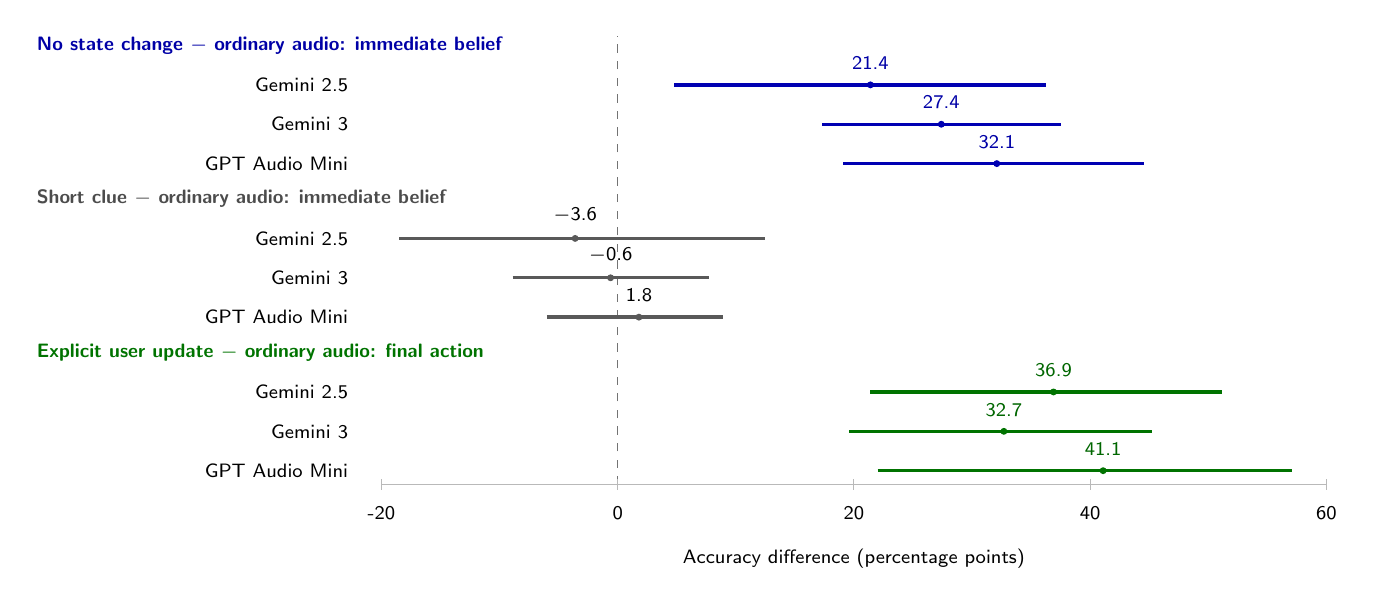
\begin{tikzpicture}[x=1.5mm,y=5mm,font=\sffamily\scriptsize]
    \draw[dashed,black!55] (0,-1.15) -- (0,10.25);
    \draw[gray!55] (-20,-1.15) -- (60,-1.15);
    \foreach \x in {-20,0,20,40,60} {
      \draw[gray!55] (\x,-1.28) -- (\x,-1.02);
      \node[below=1mm] at (\x,-1.28) {\x};
    }

    \node[anchor=west,font=\sffamily\scriptsize\bfseries,text=blue!65!black] at (-50,10) {No state change $-$ ordinary audio: immediate belief};
    \node[anchor=east] at (-22,9) {Gemini 2.5};
    \node[anchor=east] at (-22,8) {Gemini 3};
    \node[anchor=east] at (-22,7) {GPT Audio Mini};
    \draw[very thick,blue!70!black] (4.8,9) -- (36.3,9); \fill[blue!70!black] (21.4,9) circle (1.25pt); \node[above=0.7mm,text=blue!65!black] at (21.4,9) {21.4};
    \draw[very thick,blue!70!black] (17.3,8) -- (37.5,8); \fill[blue!70!black] (27.4,8) circle (1.25pt); \node[above=0.7mm,text=blue!65!black] at (27.4,8) {27.4};
    \draw[very thick,blue!70!black] (19.1,7) -- (44.6,7); \fill[blue!70!black] (32.1,7) circle (1.25pt); \node[above=0.7mm,text=blue!65!black] at (32.1,7) {32.1};

    \node[anchor=west,font=\sffamily\scriptsize\bfseries,text=black!70] at (-50,6.1) {Short clue $-$ ordinary audio: immediate belief};
    \node[anchor=east] at (-22,5.1) {Gemini 2.5};
    \node[anchor=east] at (-22,4.1) {Gemini 3};
    \node[anchor=east] at (-22,3.1) {GPT Audio Mini};
    \draw[very thick,black!65] (-18.5,5.1) -- (12.5,5.1); \fill[black!65] (-3.6,5.1) circle (1.25pt); \node[above=0.7mm] at (-3.6,5.1) {$-$3.6};
    \draw[very thick,black!65] (-8.9,4.1) -- (7.7,4.1); \fill[black!65] (-0.6,4.1) circle (1.25pt); \node[above=0.7mm] at (-0.6,4.1) {$-$0.6};
    \draw[very thick,black!65] (-6.0,3.1) -- (8.9,3.1); \fill[black!65] (1.8,3.1) circle (1.25pt); \node[above=0.7mm] at (1.8,3.1) {1.8};

    \node[anchor=west,font=\sffamily\scriptsize\bfseries,text=green!45!black] at (-50,2.2) {Explicit user update $-$ ordinary audio: final action};
    \node[anchor=east] at (-22,1.2) {Gemini 2.5};
    \node[anchor=east] at (-22,0.2) {Gemini 3};
    \node[anchor=east] at (-22,-0.8) {GPT Audio Mini};
    \draw[very thick,green!45!black] (21.4,1.2) -- (51.2,1.2); \fill[green!45!black] (36.9,1.2) circle (1.25pt); \node[above=0.7mm,text=green!40!black] at (36.9,1.2) {36.9};
    \draw[very thick,green!45!black] (19.6,0.2) -- (45.2,0.2); \fill[green!45!black] (32.7,0.2) circle (1.25pt); \node[above=0.7mm,text=green!40!black] at (32.7,0.2) {32.7};
    \draw[very thick,green!45!black] (22.0,-0.8) -- (57.1,-0.8); \fill[green!45!black] (41.1,-0.8) circle (1.25pt); \node[above=0.7mm,text=green!40!black] at (41.1,-0.8) {41.1};
    \node[below=7mm] at (20,-1.15) {Accuracy difference (percentage points)};
  \end{tikzpicture}
  \caption{Matched control effects with 95\% intervals computed across the 14 domains. Positive values favor the named intervention. Suppressing state change improves belief estimates, shortening clue distance does not, and directly reporting a user-driven update improves the final decision.}
  \label{fig:mechanism-effects}
\end{figure*}

\subsection{Direct state evidence restores belief and action}

In the explicit user-update condition, the user changes the shared state during the gap and the resumed speech directly reports the resulting outcome. Relative to the ordinary, partly implicit transition, immediate belief accuracy improved by 33.3--36.9 points and final-action accuracy improved by 32.7--41.1 points across all three models (all $p\leq.0044$). Thus, the models can revise after a gap when the new state is stated plainly. The contrast changes both the event source and how directly its outcome is described, so it supports an evidence-availability interpretation rather than a claim that user-driven events are intrinsically easier.

\subsection{The clue can change belief without changing the decision}

Restoring the causal clue improved immediate state estimates for all three models (Table~\ref{tab:clue-effects}). The effect is reliable for Gemini 3 and GPT Audio Mini and borderline under the exact domain-level test for Gemini 2.5. Final-action accuracy, however, improved only for the two Gemini models. GPT Audio Mini assigned more accurate post-gap beliefs when given the clue but did not convert that information into the correct action. This model-level dissociation demonstrates why clue validity and action accuracy should be measured separately.

\begin{table*}[t]
  \centering
  \footnotesize
  \setlength{\tabcolsep}{7pt}
  \renewcommand{\arraystretch}{1.12}
  \caption{Paired effect of restoring the causal clue. Effects are percentage points with 95\% domain-clustered intervals. Positive values mean that the clue improved performance.}
  \label{tab:clue-effects}
  \begin{tabular}{@{}lrrrr@{}}
    \toprule
    \dualcolhead{Model} & \dualcolhead{Immediate-belief effect} & \dualcolhead{$p$} & \dualcolhead{Final-action effect} & \dualcolhead{$p$} \\
    \midrule
    Gemini 2.5 Flash & +9.5 [1.8, 17.3] & .0532 & +10.1 [3.6, 17.3] & .0195 \\
    Gemini 3 Flash & +19.1 [8.3, 30.4] & .0093 & +20.2 [9.5, 30.4] & .0059 \\
    GPT Audio Mini & +13.7 [6.0, 21.4] & .0088 & $-$4.8 [$-$14.3, 5.4] & .4336 \\
    \bottomrule
  \end{tabular}
\end{table*}

The branch-pair test is stricter still: a model must answer both counterfactual versions correctly. Gemini 2.5 chose both final actions correctly in 11.9\% of pairs with the clue and 1.2\% after removal; Gemini 3 achieved 16.7\% and 3.6\%, respectively. These low absolute rates show that occasionally using the clue is easier than applying the rule consistently across both branches.

\subsection{Written context improves state estimates more consistently than actions}

Immediately after the gap, transcript conditioning improved all-state belief accuracy by 12.5 points for Gemini 2.5 and 13.1 points for Gemini 3. The latter paired effect was reliable ($p=.0127$); the former was directionally similar but uncertain ($p=.1104$). Final-action accuracy changed by only 0.6 and 11.3 points, with both intervals crossing zero. The clearest transcript effect therefore concerns the state estimate. This comparison is between accumulated audio replay and a serialized written history.

\subsection{Spoken-delivery and failure diagnostics}

The prosody conditions do not yet support a positive grounding claim. Among pairs with valid style responses, accuracy on both matched deliveries was 1.4\% for Gemini 2.5, 6.0\% for Gemini 3, and 2.2\% for GPT Audio Mini, compared with a 6.2\% random pair baseline. The directional high-versus-low style contrasts all had intervals crossing zero. Because the one-author listening audit is not complete, these results cannot distinguish model insensitivity from an insufficiently recognizable synthetic-speech manipulation. We report the conditions for completeness but do not use them as evidence for the benchmark's central claim.

Across all conditions, the automatic diagnostics marked an incorrect state belief in 83.5--95.9\% of failed trajectories. Early-clue loss appeared in 31.2--52.8\%. On the 21 audited failures, the automatic tags achieved 83.8\% precision, 55.4\% recall, and 0.667 micro F1; exact tag-set agreement was 33.3\%. The author confirmed all 20 automatically identified state-belief errors, giving that tag 100\% precision and recall in the audited sample. Narrower behavioral tags had lower recall, including repeated action (0/6), action-selection failure (1/6), and state-synchronization failure (1/5). We use the state-belief tag as the supported aggregate diagnostic and treat the narrower tags as provisional.

\FloatBarrier
\section{Discussion and Limitations}

The replicated control pattern is the central result. All three systems form substantially better state estimates when the world remains unchanged and recover both belief and action when a user-driven outcome is stated directly. Merely shortening clue distance does not help. Together, these results are consistent with a failure to infer a partly observed transition, as opposed to a generic inability to hear the dialogue or remember an earlier fact. The clue ablation adds a second diagnostic: GPT Audio Mini uses the clue in its reported belief but not its action, while the Gemini models show clue effects in both. Endpoint accuracy alone would collapse these distinct behaviors.

This target differs from EchoChain's online revision during interrupted speech and from the end-to-end completion emphasis of $\tau$-Voice, EVA-Bench, and VAmoS. We present a combination of a delayed executable transition, a matched clue intervention, and probability reports scored against the same realized world. The current evidence supports that mechanism-level diagnostic; a potential next step is to mimic natural full-duplex conversation.

Several limitations remain. Synthetic speech does not establish robustness to natural voices, accents, noise, or disfluency. The no-change and explicit-user controls necessarily alter what the resumed utterance can truthfully reveal, so they localize the combined inference burden without necessarily isolating a single acoustic variable. Transcript results cover only the Gemini models and change both interface and context representation. The belief-only checkpoint is shown back to the model before its final decision, so final-action accuracy describes belief-elicited behavior. One author audited the construction sample and failure tags; independent human performance and inter-rater agreement remain unmeasured. Finally, prosody should not be fully promoted until undergoing a separate audit process.

\section{Conclusion}

\benchmark evaluates whether an audio-conditioned agent keeps its view of the world synchronized across a delayed, partly observed transition. Its deterministic environment connects each early clue and action to a realized state, belief target, and required next decision. Across 4,368 trajectories, the models were substantially more successful when no transition occurred or when the changed state was stated directly, while a short clue distance did not resolve the failure. The benchmark therefore exposes a transition-inference gap and reveals belief--action disagreements that task completion alone cannot diagnose.

\bibliographystyle{plainnat}
\bibliography{references}

\appendix
\section{Worked causal-pair example}
\label{app:worked-example}

Table~\ref{tab:flight-example} shows the core intervention using a travel scenario. The spoken rule is the same in both branches: a departure delay at least as long as the Denver connection window makes the onward flight impossible unless it is protected. The two conversations differ only in the early answer about the connection window. After the first action, the simulator applies a 120-minute delay. The resumed words disclose the delay but not the resulting connection status. A model must combine the earlier clue with the rule to infer the state and choose the final action.

\begin{table}[htbp]
  \centering
  \footnotesize
  \setlength{\tabcolsep}{5pt}
  \renewcommand{\arraystretch}{1.14}
  \caption{A matched causal pair. The early clue changes the realized state and correct action while the post-gap words remain fixed.}
  \label{tab:flight-example}
  \begin{tabularx}{\textwidth}{@{}Q{0.16\textwidth}ZZ@{}}
    \toprule
    \dualcolhead{Element} & \dualcolhead{Short connection branch} & \dualcolhead{Long connection branch} \\
    \midrule
    Early clue & ``There are only ninety minutes between the flights in Denver.'' & ``There are four hours between the flights in Denver.'' \\
    Shared event & \multicolumn{2}{>{\raggedright\arraybackslash}p{0.77\textwidth}@{}}{Departure becomes delayed by 120 minutes.} \\
    Shared resumed words & \multicolumn{2}{>{\raggedright\arraybackslash}p{0.77\textwidth}@{}}{``The departure is now delayed by 120 minutes, but the notice does not show my connection status. Based on the connection time I mentioned earlier, what should we do next?''} \\
    Realized state & Connection missed & Connection remains viable \\
    Correct action & Protect the later segment and offer a compatible alternative & Conclude that the operation succeeded and close the request \\
    \bottomrule
  \end{tabularx}
\end{table}

The clue-removed condition replaces either early answer with the same uninformative sentence. The remaining public dialogue, synthetic voices, post-gap words, action descriptions, and randomized option order are shared within the pair. Because both branches then present the same evidence but require different answers, a clue-independent policy cannot exceed 50\% expected final-action accuracy on a balanced pair.

\section{Condition definitions}
\label{app:conditions}

The benchmark registers nine conditions, summarized in Table~\ref{tab:conditions}. Five test the central state-synchronization mechanism; the others examine user-driven change and spoken delivery. All nine were evaluated for both Gemini models. GPT Audio Mini was evaluated on the eight audio conditions.

\begin{table}[htbp]
  \centering
  \footnotesize
  \setlength{\tabcolsep}{5pt}
  \renewcommand{\arraystretch}{1.12}
  \caption{The nine controlled conditions and the factor changed in each one.}
  \label{tab:conditions}
  \begin{tabularx}{\textwidth}{@{}Q{0.20\textwidth}Q{0.17\textwidth}Z@{}}
    \toprule
    \dualcolhead{Condition} & \dualcolhead{Status} & \dualcolhead{Intervention} \\
    \midrule
    Full audio & Three models & Replay the accumulated visible conversation as audio; apply the ordinary gap event. \\
    Transcript only & Two Gemini models & Present the same visible conversation as speaker-labeled text. \\
    Clue removed & Three models & Replace the causal clue with an uninformative answer without changing turn count. \\
    No state change & Three models & Advance through the gap without applying the external state-changing event. \\
    Short distance & Three models & Move the clue pair immediately before the first evaluated decision. \\
    Explicit user update & Three models & Let the user change the shared state while the agent is absent and report the result on return. \\
    Neutral audio & Three models & Render the resumed utterance with neutral delivery. \\
    High prosody & Three models & Render the same words with the pair's higher-intensity delivery and score response approach. \\
    Low prosody & Three models & Render the same words with the pair's lower-intensity delivery and score response approach. \\
    \bottomrule
  \end{tabularx}
\end{table}

\section{Complete condition results}
\label{app:complete-results}

Table~\ref{tab:all-results} reports every model--condition cell. The main text emphasizes matched effects because raw condition differences can combine several changes in evidence and dynamics.

\begin{table*}[htbp]
  \centering
  \scriptsize
  \setlength{\tabcolsep}{5pt}
  \renewcommand{\arraystretch}{1.04}
  \caption{Complete condition results (percent). Belief is all-state top-choice accuracy immediately after the gap. Strict success requires both actions and all three belief checkpoints.}
  \label{tab:all-results}
  \begin{tabular}{@{}llrrrrr@{}}
    \toprule
    \dualcolhead{Model} & \dualcolhead{Condition} & \dualcolhead{$n$} & \dualcolhead{First action} & \dualcolhead{Final action} & \dualcolhead{Belief after gap} & \dualcolhead{Strict} \\
    \midrule
    Gemini 2.5 & Ordinary audio & 168 & 69.6 & 35.1 & 39.3 & 1.2 \\
    Gemini 2.5 & No state change & 168 & 67.9 & 38.7 & 60.7 & 8.9 \\
    Gemini 2.5 & Short clue & 168 & 63.7 & 35.7 & 35.7 & 1.8 \\
    Gemini 2.5 & Clue removed & 168 & 59.5 & 25.0 & 29.8 & 1.2 \\
    Gemini 2.5 & Transcript & 168 & 77.4 & 35.7 & 51.8 & 10.1 \\
    Gemini 2.5 & Neutral audio & 168 & 64.9 & 31.5 & 32.7 & 0.6 \\
    Gemini 2.5 & Explicit user update & 168 & 63.7 & 72.0 & 72.6 & 17.9 \\
    Gemini 2.5 & High prosody & 168 & 68.5 & 36.9 & 37.5 & 0.6 \\
    Gemini 2.5 & Low prosody & 168 & 63.7 & 32.1 & 35.7 & 3.6 \\
    \addlinespace
    Gemini 3 & Ordinary audio & 168 & 80.4 & 47.0 & 51.2 & 14.9 \\
    Gemini 3 & No state change & 168 & 75.0 & 48.2 & 78.6 & 21.4 \\
    Gemini 3 & Short clue & 168 & 66.1 & 42.3 & 50.6 & 11.9 \\
    Gemini 3 & Clue removed & 168 & 66.7 & 26.8 & 32.1 & 3.6 \\
    Gemini 3 & Transcript & 168 & 84.5 & 58.3 & 64.3 & 21.4 \\
    Gemini 3 & Neutral audio & 168 & 78.0 & 45.2 & 54.2 & 10.7 \\
    Gemini 3 & Explicit user update & 168 & 75.0 & 79.8 & 85.1 & 22.0 \\
    Gemini 3 & High prosody & 168 & 74.4 & 44.6 & 51.2 & 0.6 \\
    Gemini 3 & Low prosody & 168 & 72.0 & 40.5 & 53.0 & 2.4 \\
    \addlinespace
    GPT Audio Mini & Ordinary audio & 168 & 65.5 & 22.0 & 31.0 & 0.0 \\
    GPT Audio Mini & No state change & 168 & 61.3 & 21.4 & 63.1 & 3.0 \\
    GPT Audio Mini & Short clue & 168 & 66.7 & 20.8 & 32.7 & 1.2 \\
    GPT Audio Mini & Clue removed & 168 & 55.4 & 26.8 & 17.3 & 0.6 \\
    GPT Audio Mini & Neutral audio & 168 & 63.1 & 19.0 & 32.1 & 0.6 \\
    GPT Audio Mini & Explicit user update & 168 & 65.5 & 63.1 & 67.9 & 8.9 \\
    GPT Audio Mini & High prosody & 168 & 60.7 & 19.6 & 30.4 & 0.0 \\
    GPT Audio Mini & Low prosody & 168 & 60.7 & 20.2 & 40.5 & 0.6 \\
    \bottomrule
  \end{tabular}
\end{table*}

\section{Belief reports in plain language}
\label{app:beliefs}

The model is not asked to invent a hidden state. At each checkpoint, it receives a short, scenario-specific list of possible values and a one-sentence explanation of each value. It assigns probabilities that sum to one. For the travel example, the two reported variables are:

\begin{itemize}
  \item \textbf{Connection status:} \emph{at risk if delayed} means the connection is presently possible but a sufficiently long future delay would break it; \emph{missed} means the present delay is at least the connection window; \emph{protected} means a confirmed rebooking preserves the onward journey; and \emph{viable} means the planned connection remains feasible.
  \item \textbf{Causal alignment:} \emph{misaligned} means the earlier fact conflicts with the completion rule; \emph{aligned} means it satisfies that rule. In the travel pair, these correspond to the ninety-minute and four-hour connection windows. The prompt defines both labels but does not reveal which one is true.
\end{itemize}

Checkpoint 0 is compared with the state immediately before the first action. Checkpoint 1 is compared with the realized state immediately after the resumed observation. Checkpoint 2 is collected with the final action and checks whether reflection changed the state estimate. This creates a short belief trajectory rather than a single retrospective answer.

\section{Model request structure}
\label{app:prompt-structure}

Ordinary conversational turns ask only for a natural-language reply. At an evaluated decision, the request contains five labeled action descriptions, the possible values and explanations for each belief variable, and a request for a probability distribution and revalidation flag. Immediately after the gap, the action menu is withheld so that checkpoint 1 measures state interpretation before the final choices are shown. The final request then supplies the randomized menu and asks for the second post-gap belief report and final action.

Responses are stored in a structured record for automatic scoring, but the paper uses human-readable field names: selected option, confidence over possible states, whether new validation is needed, and response approach when prosody is evaluated. Missing or malformed fields are counted separately from substantive state errors.

\section{Metric definitions}
\label{app:metrics}

Table~\ref{tab:metric-definitions} gives the complete metric set. The main paper emphasizes component accuracies and paired effects because they are easiest to interpret. Probability-quality measures are retained for calibration analysis and reproducibility.

\begin{table}[htbp]
  \centering
  \footnotesize
  \setlength{\tabcolsep}{5pt}
  \renewcommand{\arraystretch}{1.12}
  \caption{Metrics computed from each trajectory.}
  \label{tab:metric-definitions}
  \begin{tabularx}{\textwidth}{@{}Q{0.25\textwidth}Z@{}}
    \toprule
    \dualcolhead{Metric} & \dualcolhead{Meaning} \\
    \midrule
    First-action accuracy & Whether the pre-gap action matches the action required by the initial state. \\
    Final-action accuracy & Whether the post-gap action matches the action required by the realized state. \\
    Belief accuracy & Whether the highest-probability value is correct for every requested state variable at a checkpoint. \\
    Truth probability & The probability assigned to the correct state value; unlike top-choice accuracy, this preserves confidence information. \\
    Negative log-likelihood & Penalizes low probability on the truth, with a particularly large penalty for confident errors. \\
    Brier score & Squared distance between the reported probabilities and the correct one-hot state; lower is better. \\
    Normalized entropy & How diffuse the reported distribution is after accounting for the number of possible values. \\
    Revision gain & Change in probability assigned to the realized state after the resumed observation. \\
    Stale mass & Probability retained on the state that held before the gap but no longer holds. \\
    Belief--action consistency & Whether the selected action is appropriate for the state the model itself considered most likely. \\
    Strict success & Both actions and all three belief checkpoints are correct in the same trajectory. \\
    \bottomrule
  \end{tabularx}
\end{table}

For matched condition comparisons, each scenario is paired with the same scenario under the intervention. The reported effect is the mean within-domain accuracy difference, and confidence intervals and permutation tests use the 14 domains as the independent units. This avoids treating multiple variants of one domain as unrelated evidence.

\section{Scenario coverage}
\label{app:coverage}

Table~\ref{tab:scenario-coverage} lists the state variable controlled by the early fact in each domain. Every causal pair has one branch that satisfies the stated completion rule and one that requires a domain-specific recovery action.

\begin{table}[htbp]
  \centering
  \footnotesize
  \setlength{\tabcolsep}{4pt}
  \renewcommand{\arraystretch}{1.10}
  \caption{Domains, outcome variables, and recovery actions in the 84-scenario release.}
  \label{tab:scenario-coverage}
  \begin{tabularx}{\textwidth}{@{}Q{0.17\textwidth}Q{0.18\textwidth}Q{0.22\textwidth}Z@{}}
    \toprule
    \dualcolhead{Domain} & \dualcolhead{Outcome state} & \dualcolhead{Misaligned outcome} & \dualcolhead{Recovery action} \\
    \midrule
    Technical support & Firmware status & Stuck & Inspect persistent state \\
    Pharmacy & Claim status & Rejected & Review account configuration \\
    Travel & Connection status & Missed & Protect onward segment \\
    Banking & Dispute status & Returned unmatched & Reconcile card records \\
    Health care & Authorization status & Declined & Obtain qualifying referral \\
    Logistics & Shipment status & Returned to sender & Correct destination record \\
    Energy & Reading status & Flagged incomplete & Register all supply points \\
    Account access & Access status & Still locked & Engage identity provider \\
    Warranty & Claim state & Outside terms & Use retailer route \\
    Housing & Work-order status & Access refused & Reissue access authority \\
    Mobile service & Port status & Rejected & Align ownership record \\
    Education & Enrolment status & Held for review & Request prior-study assessment \\
    Motor insurance & Claim progress & Held for proof & Align policy records \\
    Permits & Permit status & Refused & Supply alternative proof \\
    \bottomrule
  \end{tabularx}
\end{table}

% The official NeurIPS checklist is included when checklist.tex is placed in
% this directory. It appears after the references and does not use content pages.
\IfFileExists{checklist.tex}{
  \newpage
  \input{checklist.tex}
}{}

\end{document}
